\section{Place Recognition Algorithm}
\label{sec:chap_slam_algo}

While there is quite a few articles presenting place recognition algorithms using different sensors (e.g. cameras, \gls*{gps}), the literature of such algorithms based solely on \gls*{3d} data is limited. For our place recognition analysis, we choose to use the state-of-the-art algorithm (at the time of the experiments) developed by \citet{Steder2011b}. The details of the technique are presented in the article, but for the needs of this document, we will first describe in more details some fundamental concepts used by the algorithm in Section~\ref{ssec:chap_slam_basics} and then we will give an overview of the algorithm itself in Section~\ref{ssec:chap_slam_algo}. 


\subsection{Fundamental Concepts}
\label{ssec:chap_slam_basics}

The first step to determine whether or not a place have been visited by the robot before, is to convert the data into a more convenient format for identification. The generally adopted representation is a vector of real numbers, called descriptor. A descriptor can be global, meaning that it represents the whole sample, or local, meaning that it represents a specific subregion of the sample. When using local descriptors, it is first required to determine the interest points around which they will be build. These keypoints can be fixed (e.g. division in a simple grid) or selected using more refined algorithms. A common practice is to choose keypoints in region of high gradiant (e.g. edges, corners), since these region generally contains more informations than smooth surfaces. Note that for simplicity, we might use the term \textbf{features} as a more general term for keypoints and descriptors in the remainder of this document.

The concepts of keypoints and descriptors originate from the computer vision literature, but they have been adapted for \gls*{3d} data. You can find some popular examples of features for both type of data in Table~\ref{tab:chap_slam_features_examples}. Note that some algorithms propose solutions for both keypoints detection and descriptors (e.g. SIFT, NARF), but it is not mandatory to use them together as any combination is generally valid. While all existing features are different, they were all developed with the same goals in mind:
\begin{itemize}[label=$\bullet$,noitemsep,topsep=0pt]
    \item Distinctiveness: each feature should be easily differentiable with respect to other.
    \item Repeatability: the feature values should be stable under changes including:
        \begin{itemize}[label=$\circ$,noitemsep,topsep=0pt]
            \item Transformations: any rigid transformation in the case of point clouds, including the pose of the object and the viewpoint.
            \item Noise: small variations in range measurements and occasional erroneous points.
            \item Resolution: the amount of points representing a given area.
        \end{itemize}
\end{itemize}

\begin{table}[H]
    \centering
    \begin{tabular}{@{}llll@{}}
        \toprule
        \textbf{Type of data}  & \textbf{Keypoint/descriptor} & \textbf{Name}               & \textbf{Reference} \\
        \hline
        Image                  & Keypoint                     & Harris and Stephens corners & \cite{Harris1988}  \\
        Image                  & Both                         & SIFT                        & \cite{Lowe2004}    \\
        Image                  & Both                         & SURF                        & \cite{Bay2006}     \\
        \gls*{3d}              & Descriptor                   & FPFH                        & \cite{Rusu2009}    \\
        \gls*{3d}              & Both                         & ISS                         & \cite{Yu2009}      \\
        \gls*{3d}              & Descriptor                   & SHOT                        & \cite{Tombari2010} \\
        \gls*{3d}              & Both                         & NARF                        & \cite{Steder2011a} \\
        \bottomrule
    \end{tabular}
    \caption{\todo{Might just put image examples in the text, find better layout ? Add info ?} Examples of popular descriptors and keypoints detectors for images and \gls*{3d} data. Some \gls*{2d} keypoints have been adapted for \gls*{3d} such as Harris and Stephens and SIFT.}
    \label{tab:chap_slam_features_examples}
\end{table}

For our place recognition analysis we choose to use the NARF keypoints and descriptors. In addition to being intrinsically related to the algorithm used, these features present some interesting characteristics which we will discuss briefly. For a detailed description, we recommend reading the original article \citet{Steder2011b}. The computation of those features requires a pre-processing step, which consist in converting the point cloud into a range image. The range image is a spherical projection of the points from the center of sensor. You can see examples of this data type in Figure~\ref{fig:chap_slam_range}. Certain constraints must be respected for producing such type of data. Firstly, this conversion require the acquisition to originate from a single view point, which is the case for our dataset. Another constraint is that there must be no missing point in the scan. Since this is not respected for our data, all missing points are considered as far range (i.e. the maximum range of the sensor). Finally, the resolution was adjusted so that every pixel cover the same angle in both directions. The resulting data format is a dense and uniform representation that can be processed similarly to images. Using the range images, NARF features are able to differentiate edges that are part of the boundary of objects as oppose to edges that are produced by occlusions, which is not possible using point clouds directly. This is useful in highly occluded environments such as forest, where edges caused by occlusions can produce bad features, leading to a poor representation of the environment which can reduce the place recognition performance.

\begin{figure}[H]
    \centering
    \subfloat[]{\label{fig:range_building}}{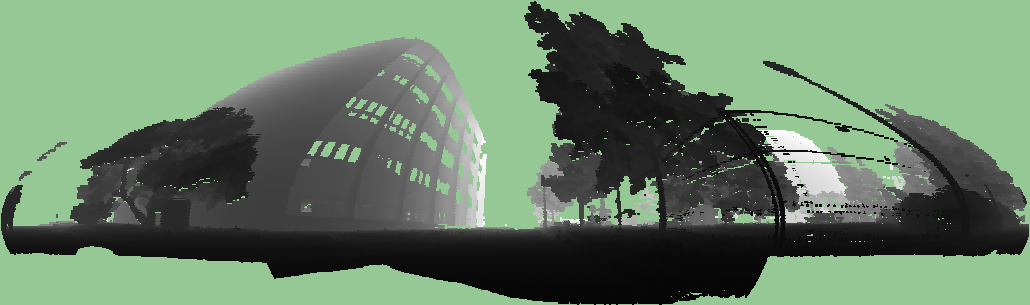
\includegraphics[width=0.995\linewidth]{img/chap_slam/range_building01.png}}\\
    \subfloat[]{\label{fig:range_forest}}{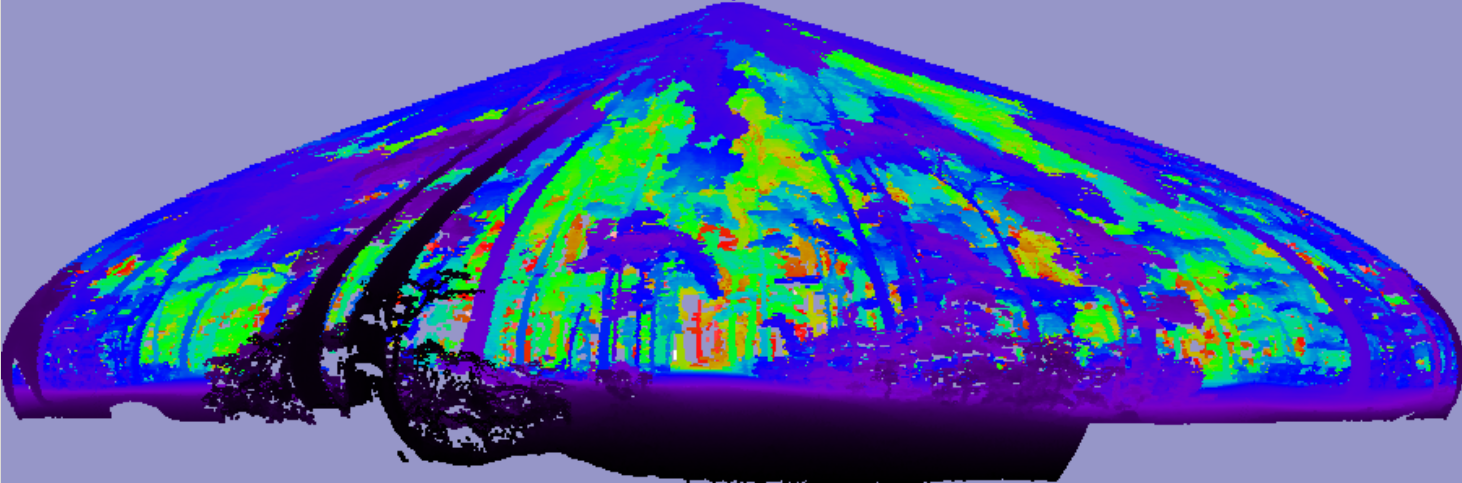
\includegraphics[width=0.995\linewidth]{img/chap_slam/range_forest01.png}}
    \caption{Examples of range images for the structured dataset \protect\subref{fig:range_building} and the unstructured dataset \protect\subref{fig:range_forest}. Note that the objects look distorted due to the projection on the plane and that the background color corresponds to the areas without laser return.}
    \label{fig:chap_slam_range}
\end{figure}

The last item we need to discuss in this subsection is the method used to compare two samples. Similarity between descriptors can generally be computed using a simple distance metric (e.g. euclidean distance). The comparison is straightforward when using a global descriptor which represent the whole sample, but when using a set of local descriptors, further processing is required. A popular solution is to convert this set of features into a single \gls*{bow}\todo{cite?} and then use this new format for comparison. The concept of \gls*{bow} was first used for documents classification. In this context, they represented a document by a vector of occurrence counts of a vocabulary. In our case, the amount of descriptors made up of real numbers is infinite and therefore cannot be used directly as words. The solution to this problem is to use a clustering algorithm such as k-means\todo{cite?} to create groups that will represent words. The vocabulary is generally created in advance using a large collection of local descriptors gathered under similar conditions. The representation in words avoids having to compare the descriptors by hand according to their distance in the space of descriptors and remove any information regarding the geometric configuration of keypoints in the samples. This is a rather general representation with which the comparison is relatively fast to compute. Another approach to compare \gls*{3d} samples consist in finding local descriptors correspondences and checking if there is a valid transformation that aligns these. The vectors of real numbers representing the features (i.e. the descriptors) will never be exactly the same, but if the distance between them is smaller than a certain threshold they will be considered as correspondences. The corresponding descriptors between two samples are then use to determine if there is a valid rigid \gls*{3d} transformation that align the underlying keypoints. This step also requires a criteria on the number of features correctly aligned, thereby identifying the samples as originating from the same place or not. This is generally achieved using the RANSAC algorithm\todo{cite?}. Figure~\ref{fig:chap_slam_features_correspondences} show keypoints from two samples as well as examples of correspondences. This second technique is more computationally expensive, but is also more discriminative.

\begin{figure}[H]
    \centering
    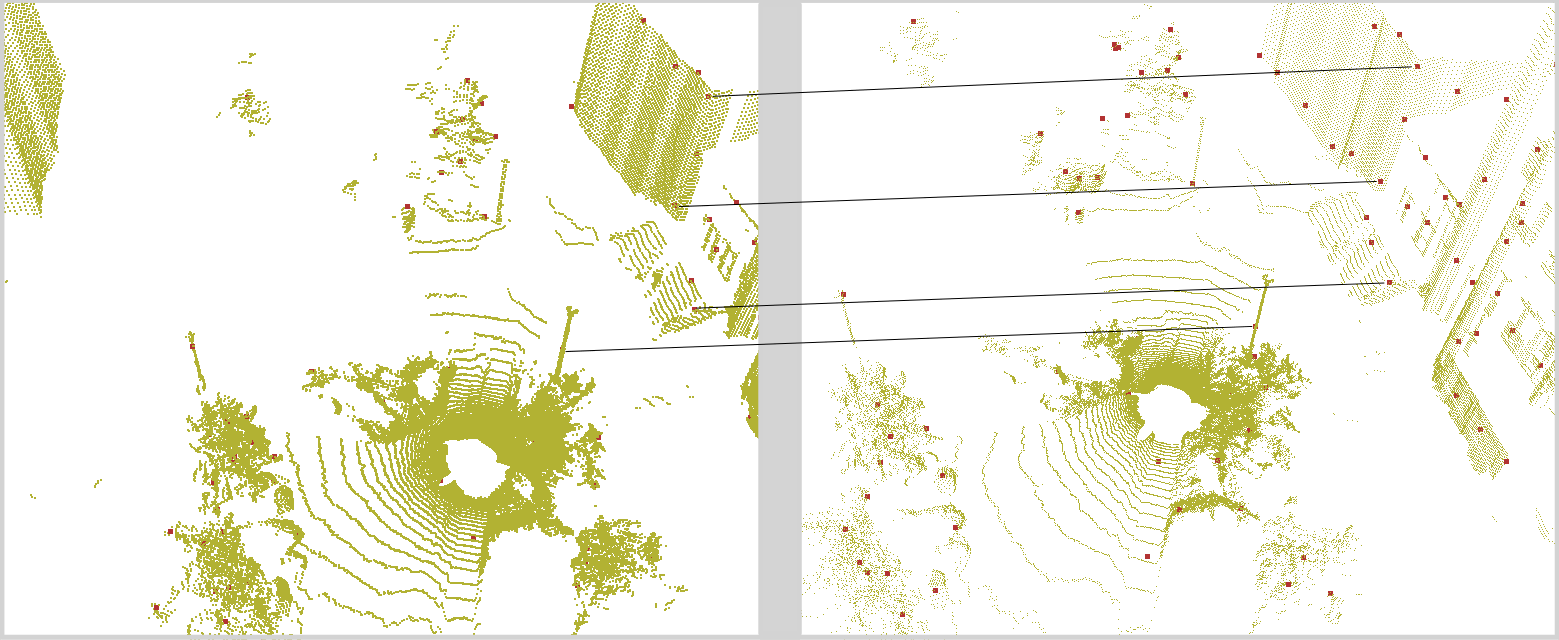
\includegraphics[width=0.995\linewidth]{img/chap_slam/features_line.png}\\
    \caption{Examples of NARF keypoints found for two different samples of the structured dataset. Black lines illustrate examples of valid correspondences found. These show stability under changes, such as viewpoint, noise and resolution.}
    \label{fig:chap_slam_features_correspondences}
\end{figure}


\subsection{Overview of the Algorithm}
\label{ssec:chap_slam_algo}

\todo{This section will give some more details about the NARF algorithm itself.}
